\section{Performance evaluation}

We use the web service example described in the previous section, figure \ref{fig:fluxions}, to compare the fluxionnal execution model, to basic Javascript implementation, listing \ref{lst:classique}.
For this evaluation against the basic implementation, we developed different version of the fluxionnal execution models using different methods for chaining fluxions.

\begin{itemize}
	\item[\textbf{Chain}]
		This implementation chains fluxions one after another by a direct function call.
		It set the fluxions chain length maximum to the macimum function call stack size, and it make it impossible to interleave messages from network.

	\item[\textbf{NextTick}]
		This implementation uses the instruction \texttt{process.nextTick} to chain fluxions execution.
		This instruction makes it possible to probe network messages only every \textit{n} fluxions execution. By default \textit{n} is set to 1000.

	\item[\textbf{SetTimeout}]
		This implementation uses the instruction \texttt{setTimeout}.
		It probes network messages after every fluxion execution, thus networks messages can be interleaved between each local messages.
\end{itemize}

With these differents implementations, we want to highlight the advantages and drawbacks of the fluxionnal execution model.

\begin{figure}
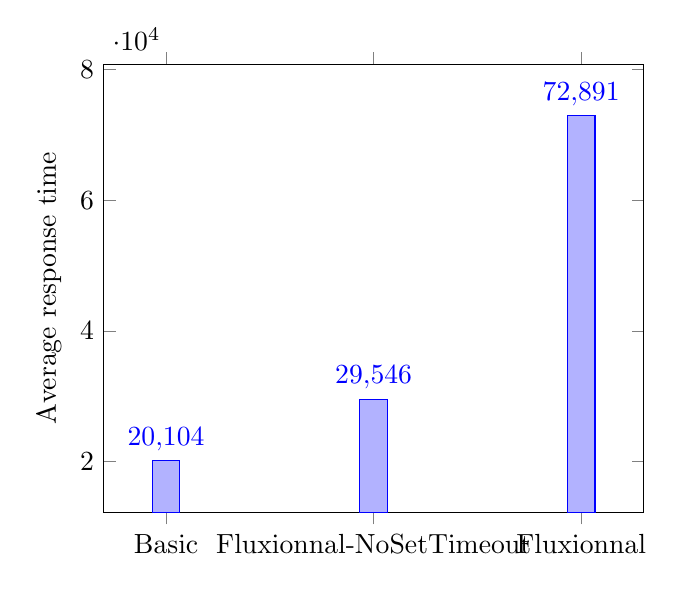
\begin{tikzpicture}
	\begin{axis} [
 		ybar,
 		enlargelimits=0.15, 
 		legend style={at={(0.5,-0.15)},anchor=north,legend columns=-1},
 		ylabel={Average response time},
 		symbolic x coords={Basic,Fluxionnal-NoSetTimeout,Fluxionnal},
 		xtick=data,
 		nodes near coords,
 		nodes near coords align={vertical}
	]
		\addplot coordinates {(Basic,20104) (Fluxionnal-NoSetTimeout,29546) (Fluxionnal,72891)};
	\end{axis}
\end{tikzpicture}
\caption{Average response time for each implementation}
\label{fig:reponsetime}
\end{figure}



We can see that the use of fluxions, from our implementation of the fluxionnal execution model increases the average response time of about 50\%, as the \textbf{Fluxionnal-NoSetTimeout} implementation aberage response time show from the \textbf{Basic} implementation.
However, the instruction \texttt{SetTimeout}, used in the original Fluxionnal execution model, increases the average response time of this implementation of about 360\%.



\TODO{}
Although, using a fluxionnal approach is a way to build an efficient distributed system we consider that the most important part of our work is to enable code transformation from a standard basic web approach to a flow of fluxions.
We show now the main code transformation we propose.